\section{Poisson solver}
\label{sec:poisson}
In this section of the lab report, we will dicuss a prallel implementation of the Poisson solver. The Poisson solver is a numerical method used to solve the Poisson equation, which is a partial differential equation that is useful in many areas of physics. \\
\subsection{Building a parallel Poisson solver}
For the first part of the exercise we follow the steps lined out in the assignment sheet. I'll comment on the steps 1 through 10 and related questions bellow. The finished implementation can be found in the appendix for this section. \\
\begin{enumerate}
    \item \textbf{Step 1:} After adding MPI_Init and MPI_Finalize, we can run the program with multiple processes.  
    \begin{figure}[H]
        \centering
        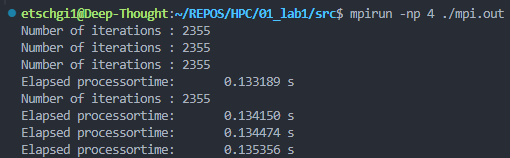
\includegraphics[width=\textwidth]{../fig/lab1/step1.png}
        \caption{MPI_Poisson after Step 1 - Running with 4 processes}
        \label{fig:poisson_step1}
    \end{figure}
\end{enumerate}